\chapter{Control System Figures}\label{A:control}
\vspace{-20pt}

\section*{Variable Output Voltage Duty Cycle Control} \label{A:control_duty}

\begin{figure}[H]
    
    \centering
    \begin{subfigure}{0.5\textwidth}
        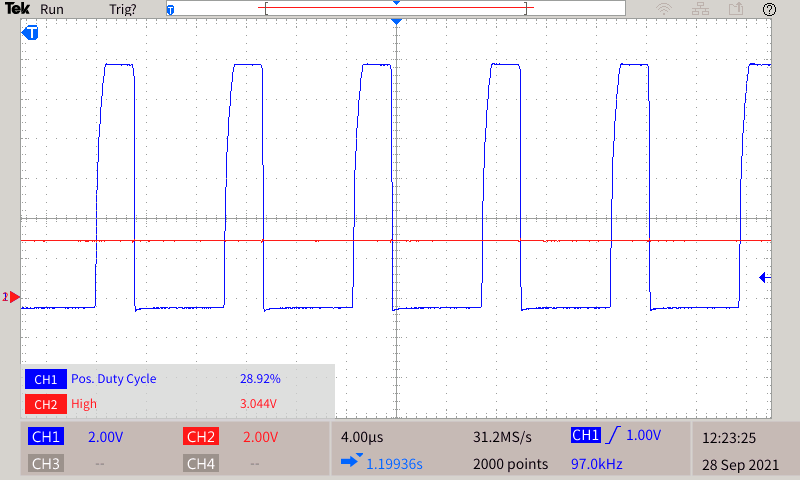
\includegraphics[width=\columnwidth]{control/duty_control/duty_3V.PNG}
        \subcaption{Controlled duty cycle of 28.9\% for a 3V DC output}
    \end{subfigure}
    \begin{subfigure}{0.5\textwidth}
        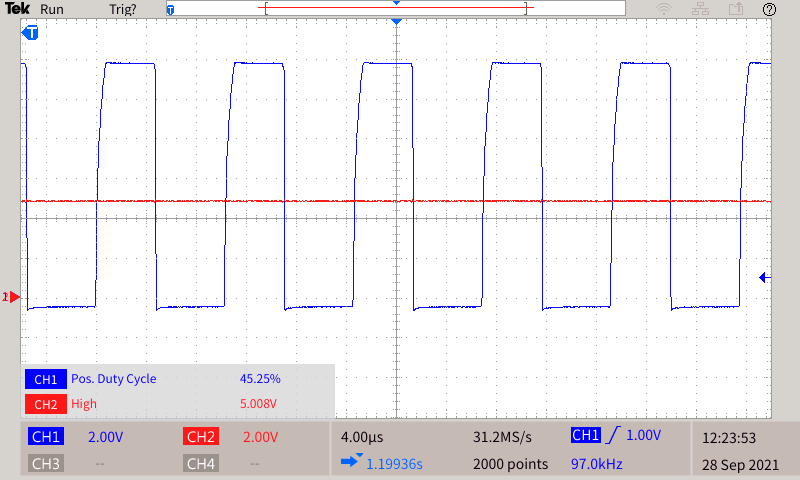
\includegraphics[width=\columnwidth]{control/duty_control/duty_5V.PNG}
        \subcaption{Controlled duty cycle of 45.25\% for a 5V DC output}
    \end{subfigure}
    \begin{subfigure}{0.5\textwidth}
        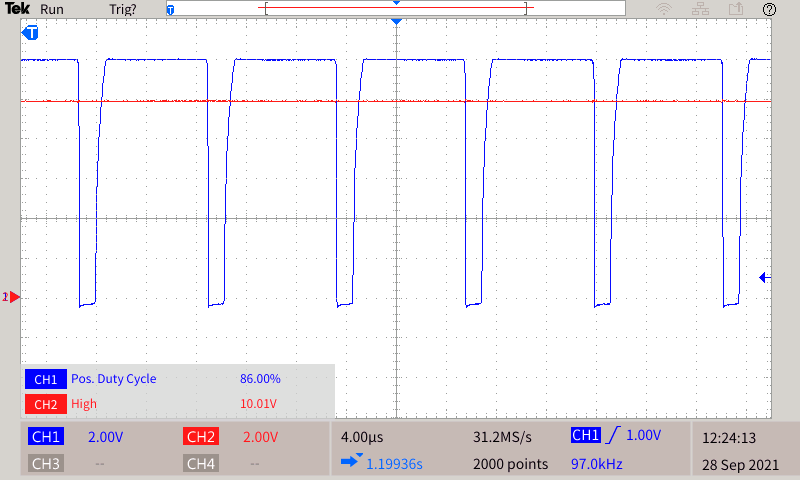
\includegraphics[width=\columnwidth]{control/duty_control/duty_10V.PNG}
        \subcaption{Controlled duty cycle of 86.0\% for a 10V DC output}
    \end{subfigure}
    \caption{PWM duty cycle controlled by the voltage output control system (Blue), achieving 3V, 5V and 10V DC (Red).}
\end{figure}

\section*{Output Voltage Control System Step Response Rise Time} \label{A:control_step_rise}
\begin{figure}[H]
    \centering
    \begin{subfigure}{0.62\textwidth}
        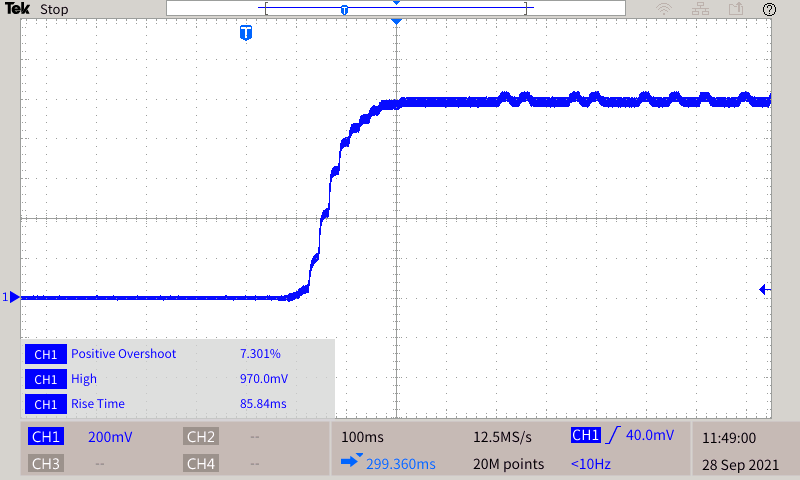
\includegraphics[width=\columnwidth]{control/step_response/voltage_control_0-1.PNG}
        \subcaption{Output voltage controller 0V to 1V step response with 86ms settleing time.}
    \end{subfigure}
    \begin{subfigure}{0.62\textwidth}
        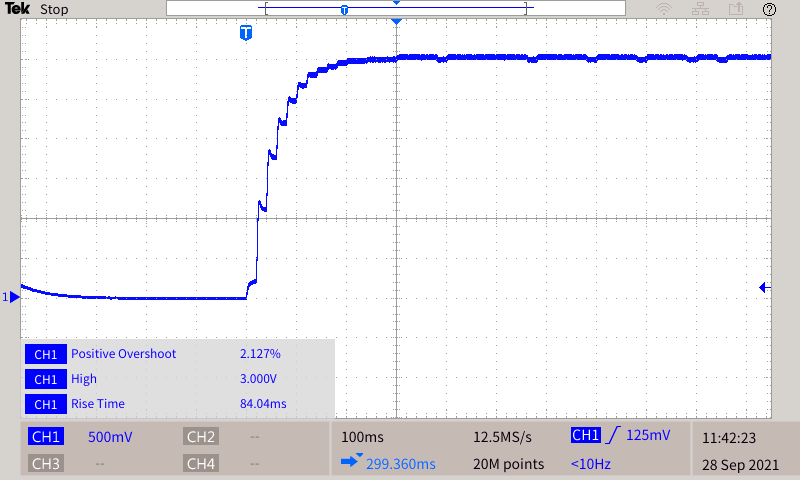
\includegraphics[width=\columnwidth]{control/step_response/voltage_control_0-3.PNG}
        \subcaption{Output voltage controller 0V to 3V step response with 84ms settleing time.}
    \end{subfigure}
    \begin{subfigure}{0.62\textwidth}
        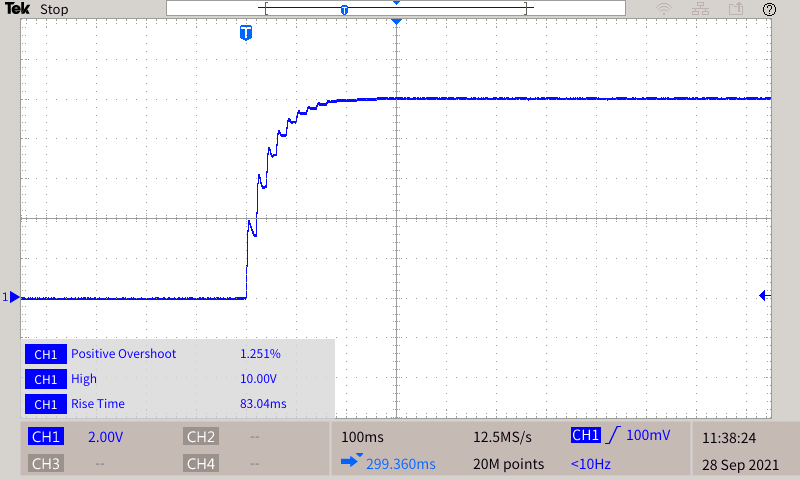
\includegraphics[width=\columnwidth]{control/step_response/voltage_control_0-10.PNG}
        \subcaption{Output voltage controller 0V to 10V step response with 83ms settleing time.}
    \end{subfigure}
    \caption{Output voltage control system step response, reacting to 1V, 3V and 10V output steps.}
\end{figure}

\section*{Output Voltage Control System Step Response Fall Time} \label{A:control_step_fall}
\begin{figure}[H]
    \centering
    \begin{subfigure}{0.7\textwidth}
        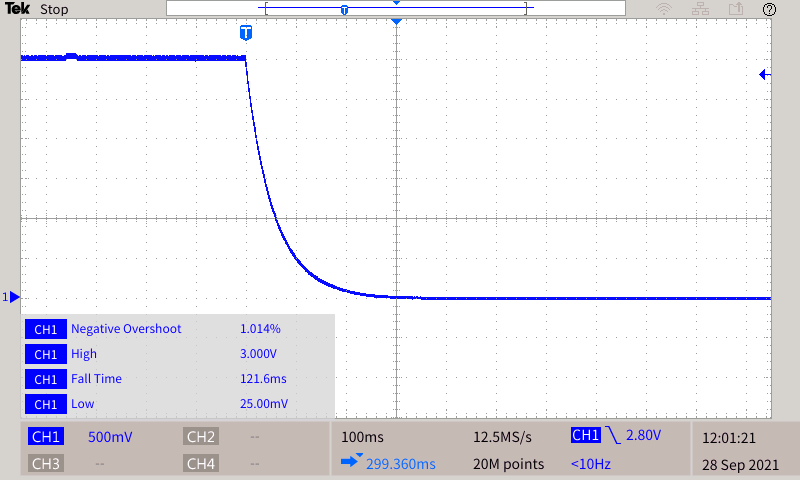
\includegraphics[width=\columnwidth]{control/step_response/voltage_control_3-0.PNG}
        \subcaption{Output voltage controller 3V to 0V step response with 121ms settleing time.}
    \end{subfigure}
    \begin{subfigure}{0.7\textwidth}
        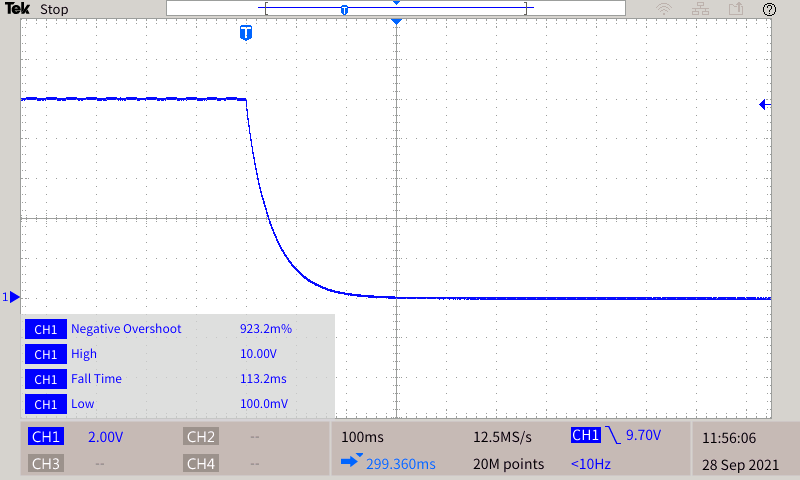
\includegraphics[width=\columnwidth]{control/step_response/voltage_control_10-0.PNG}
        \subcaption{Output voltage controller 10V to 0V step response with 113ms settleing time.}
    \end{subfigure}
    \caption{Output voltage control system step response, reacting to -3V and -10V output steps.}
\end{figure}

\section*{Output Voltage Control System with Variable Supply Voltage} \label{A:control_supply_change}
\begin{figure}[H]
    \centering
    \begin{subfigure}{0.62\textwidth}
        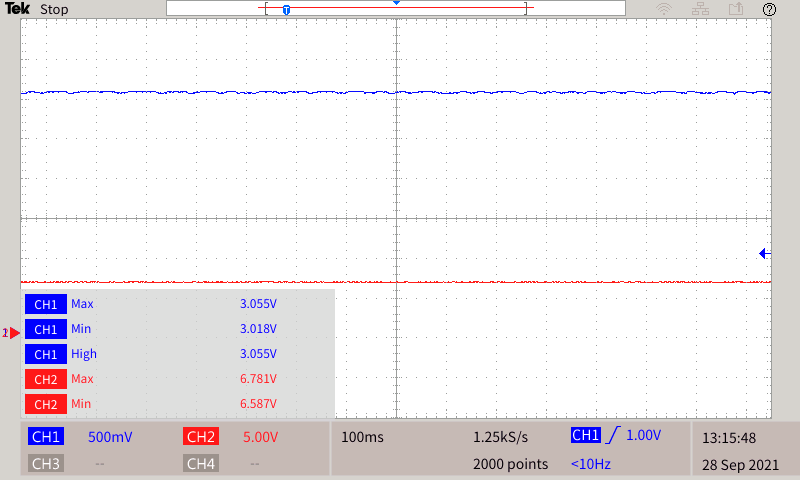
\includegraphics[width=\columnwidth]{control/variable_input/VO-3_VCC-6.PNG}
        \subcaption{Output voltage controller regulating a 6V supply (Red) for a 3V output (Blue)}
    \end{subfigure}
    \begin{subfigure}{0.62\textwidth}
        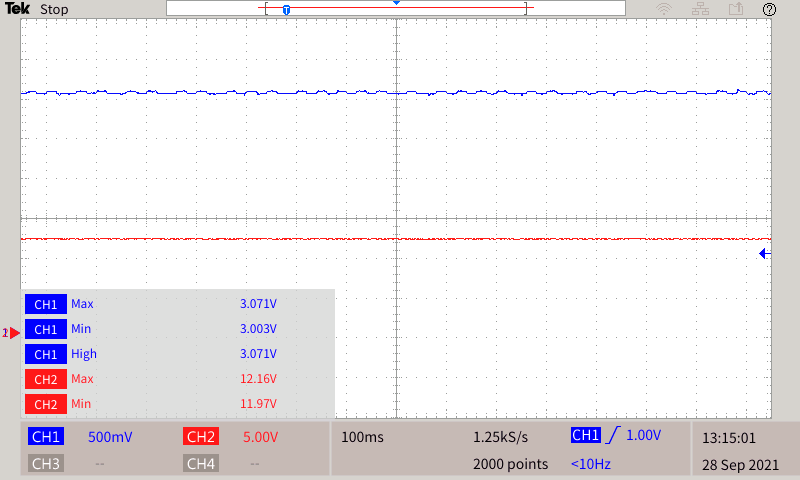
\includegraphics[width=\columnwidth]{control/variable_input/VO-3_VCC-12.PNG}
        \subcaption{Output voltage controller regulating a 12V supply (Red) for a 3V output (Blue)}
    \end{subfigure}
    \begin{subfigure}{0.62\textwidth}
        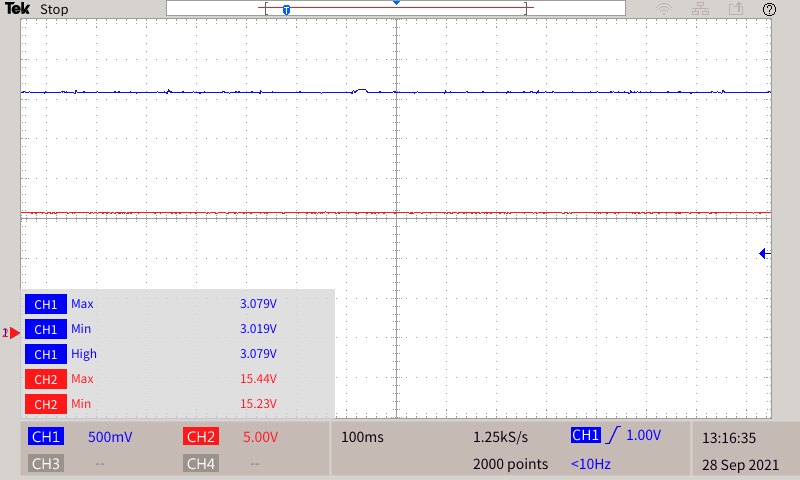
\includegraphics[width=\columnwidth]{control/variable_input/VO-3_VCC-16.PNG}
        \subcaption{Output voltage controller regulating a 16V supply (Red) for a 3V output (Blue)}
    \end{subfigure}
    \caption{Output voltage controller regulating variable supply voltages for constant output.}
\end{figure}

\section*{Output Voltage Control System Supply Voltage Step} \label{A:control_supply_step}

\begin{figure}[H]
    \begin{center}
        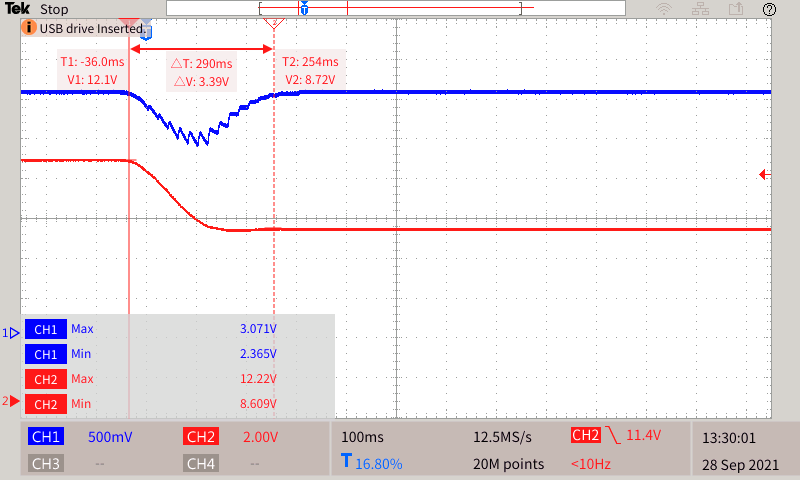
\includegraphics[width=0.9\textwidth]{control/variable_input/VCC-step_12-8.PNG}
        \caption{Output voltage controller response (Blue) to a 12V to 8V supply voltage step (Red), with a recovery time of 290ms}
    \end{center}
\end{figure}

\begin{figure}[H]
    \begin{center}
        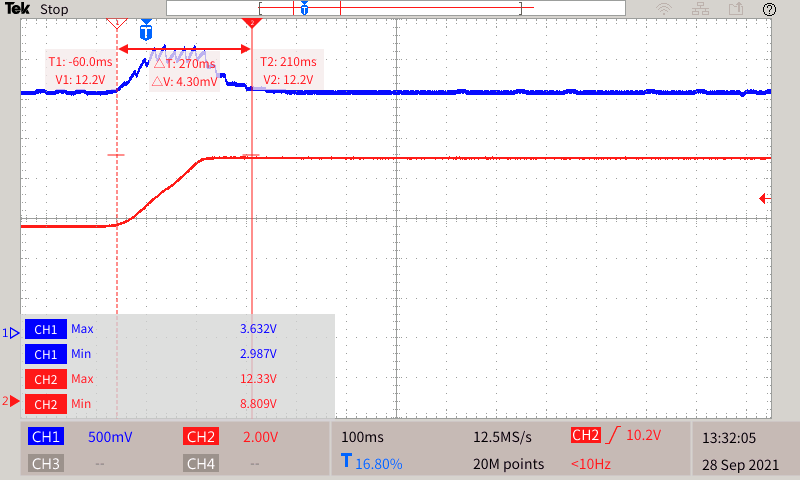
\includegraphics[width=0.9\textwidth]{control/variable_input/VCC-step_8-12.PNG}
        \caption{Output voltage controller response (Blue) for a 8V to 12V supply voltage step (Red), with a recovery time of 270ms}
    \end{center}
\end{figure}